\chapter{Control Unit}
The Control Unit is the component that directs the operations of the processor. \\
There are different possibilities for its implementation and we choose the hardwired one: \\
the control hardware is a finite state machine that switches from a state to another at every clock cycle, generating a sequence of individual bits that represent the control signals (i.e. control words). \\
\\
\begin{figure}[h!]
	\centering
	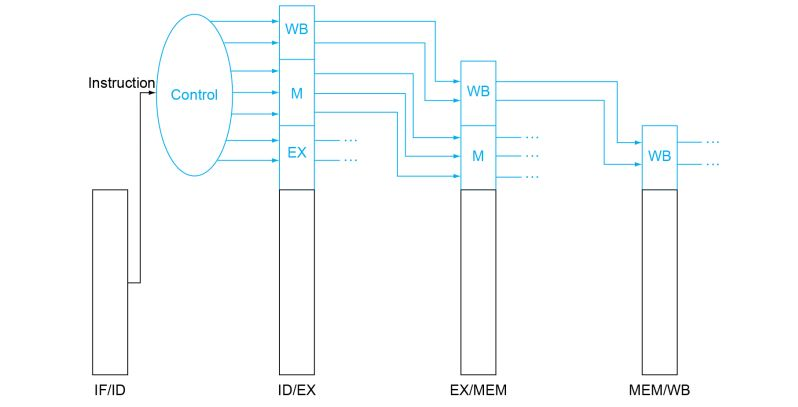
\includegraphics[width=12cm]{./images/structure_CU}
	\caption{General CU structure}
	\label{fig3.1}
\end{figure}

\section{Control Word Generation}
The component receives as an input the instruction and based on its Opcode, the control unit decides which control word (CW) has to be sent to the output. \\
This selection is based on the bits in position 2, 4, 5, 6; and once concatenated together, they identify each instruction uniquely.\\
These bits are used to access to the matrix that generates the corresponding CW.\\
\begin{figure}[h!]
	\centering
	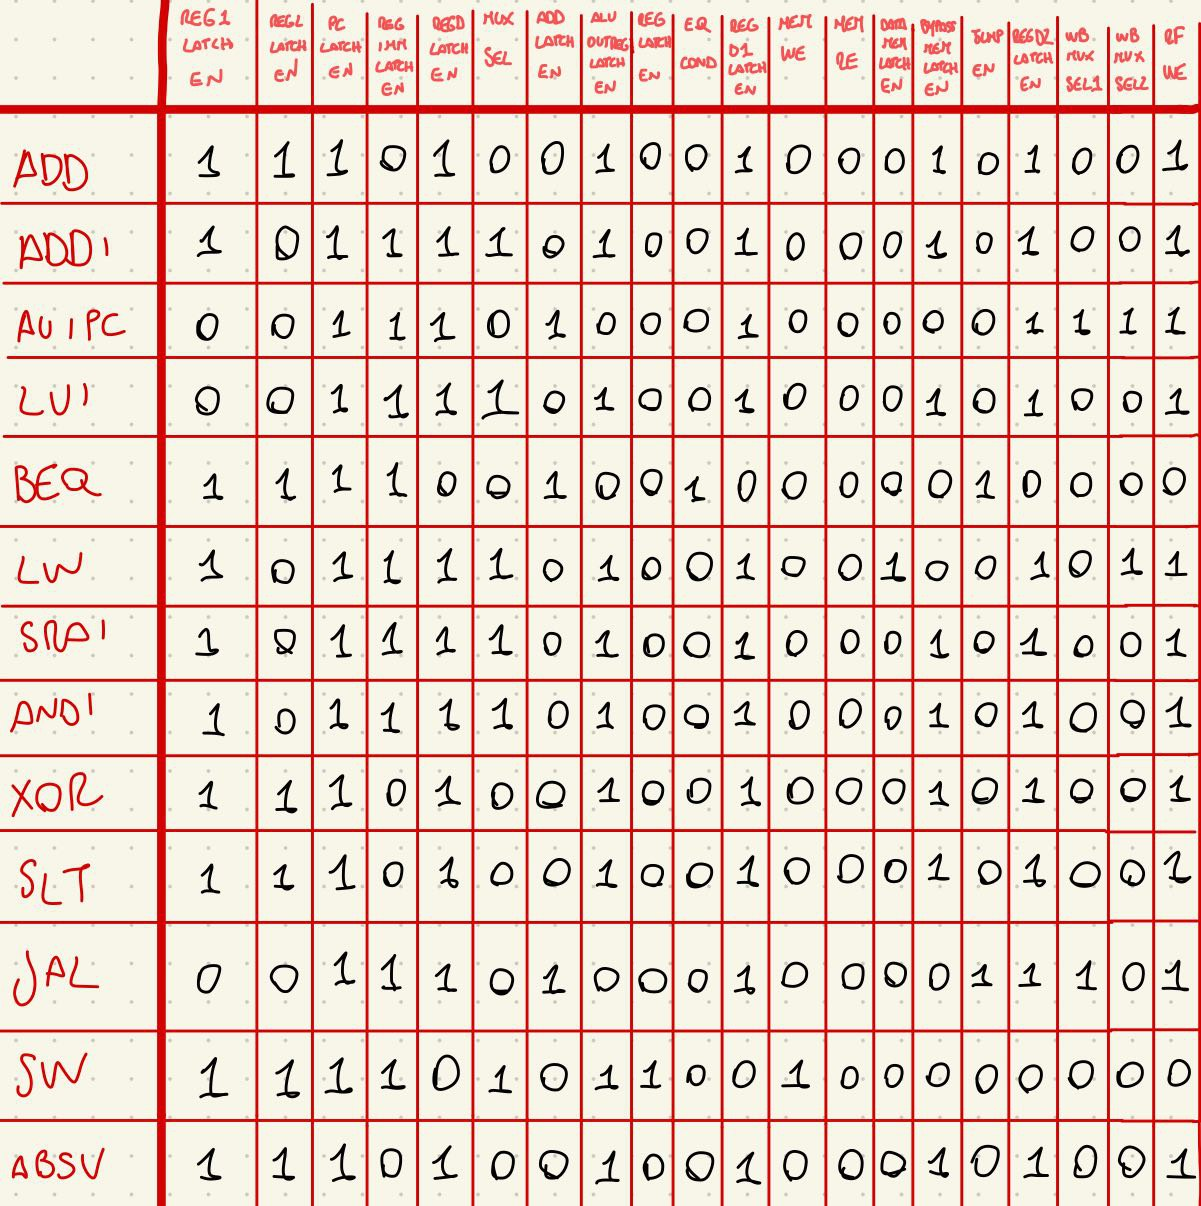
\includegraphics[width=16cm]{./images/control_signals}
	\caption{Control signal of each instruction}
	\label{fig3.3}
\end{figure}
Each instruction has its own control signals, and they are the same for instructions belonging to the same class (however, there are some exceptions of signals that belong to the same class but have different control signals):\\

\begin{itemize}
	\item I-type (ADDI, SRAI, ANDI);
	\item LW (I-type);
	\item R-type (ADD, XOR, SLT);
	\item B-type (BEQ);
	\item J-type (JAL);
	\item S-type (SW);
	\item AUIPC (U-type);
	\item LUI (U-type);		
\end{itemize}
\section{ALU Opcode generation}
The second process present in the CU description is the one dedicated to the generation of the code destinated to the ALU, in order to determine its behavior.
Its sensitivity list contains the instruction's OPCODE, the instruction's FUNCT and it follows the scheme below:\\
\\
\begin{itemize}
	\item I-type -$>$ OPCODE = "0010011" :
		\begin{itemize}
			\item ADDI -$>$ FUNCT = "000";
			\item SRAI -$>$ FUNCT = "101";
			\item ANDI -$>$ FUNCT = "111";
		\end{itemize}
	\item LW (I-type) -$>$ OPCODE = "0000011";
	\item R-type -> OPCODE = "0110011":
		\begin{itemize}
			\item ADD -$>$ FUNCT = "000";
			\item XOR -$>$ FUNCT = "100";
			\item SLT -$>$ FUNCT = "010";
		\end{itemize}
	\item B-type (BEQ) -$>$ OPCODE = "1100011";
	\item J-type (JAL) -$>$ OPCODE = "1101111";
	\item S-type (SW) -$>$ OPCODE = "0100011";
	\item AUIPC (U-type) -$>$ OPCODE = "0010111";
	\item LUI (U-type) -$>$ OPCODE = "0110111";		
\end{itemize}

\section{Absolute value (ABSV))}

For the absolute value we decided to use the same instruction bit of the SLTIU that is not used in our lite version of the RISC-V. In doing so, the instruction will be in the I-type family and in assembly can be easily written by giving the source register, the destination register and writing the immediate part as 0s.\\\\
For instance:\\ 
ABSV x2, x16, 0x0\\
The processor will take the value stored in register 16 of the register file, performs the absolute value operation and stores the new value in the register 2 of the register file.\\\\

\begin{itemize}
	\item I-type -$>$ OPCODE = "0010011" :
	\begin{itemize}
		\item ADDI -$>$ FUNCT = "000";
		\item SRAI -$>$ FUNCT = "101";
		\item ANDI -$>$ FUNCT = "111";
		\item  \textbf{ABSV -$>$ FUNCT = "011";}
	\end{itemize}
	\item LW (I-type) -$>$ OPCODE = "0000011";
	\item R-type -> OPCODE = "0110011":
	\begin{itemize}
		\item ADD -$>$ FUNCT = "000";
		\item XOR -$>$ FUNCT = "100";
		\item SLT -$>$ FUNCT = "010";
	\end{itemize}
	\item B-type (BEQ) -$>$ OPCODE = "1100011";
	\item J-type (JAL) -$>$ OPCODE = "1101111";
	\item S-type (SW) -$>$ OPCODE = "0100011";
	\item AUIPC (U-type) -$>$ OPCODE = "0010111";
	\item LUI (U-type) -$>$ OPCODE = "0110111";		
\end{itemize}